
\section{Verifying  \lgname programs}
\label{sec:verification}

\newcommand{\Ev}{\ensuremath{e}\xspace}
\newcommand{\EvCond}{\ensuremath{\mathit{Cond}}\xspace}
\newcommand{\EvBody}{\ensuremath{\mathit{Body}}\xspace}

%\rg{round, program transition, event execution, $\delta$-transition are all defined at this point: program transition : events executed in some order, $\delta$-transition: simulataneous advancement of time, round = program + $\delta$-transition. }
% connect to definition of e.
%make the post definition on a set.

We have built the semantics of $\lgname$ in the \K framework to enable decoupled analyses of platform-independent discrete part and the platform-dependent (dynamic) parts of distributed multi-robot systems. The \emph{events} in an $\lgname$ program define the discrete computations in the system.
The effect of a robot $i$ executing event $\Ev \in \Event$ on a configuration $\gconfig \in \pwg$,
can be seen as a $\stmtrule$ application to  $\left\langle \gconfig.S, \gconfig.\lconfig{i}, \EvBody \right\rangle $,
where $\Ev$ is \emph{``eventName: {\normalfont\bf pre:} \EvCond\ {\normalfont\bf eff:} \EvBody''}.


\subsection{Reachable configurations}

Given a set of system configurations $\gset$,
we define the following functions using the semantic rules of \refsect{semantics}:
\begin{inparaenum}[(i)]
    \item $\Post_\Ev(\gconfig,i)$ returns the set of configurations obtained by robot $i$ executing event $\Ev \in \Event$ from a configuration $\gconfig$.
%          \sayan{are events deterministic? Did we discuss somewhere?}
    \item $\Post(\gset,i)$ returns the set of configurations obtained by robot $i$ executing any event from a configuration in $\gset$.
    \item $\Post(\gset,\pvec)$ returns all configurations visited, when robots execute their events in the order $\pvec$,
          where $\pvec$ is a sequence of $p_i \in \UINS$.
    \item $\Post(\gset)$ is the union of $\Post(\gset,\pvec)$ over all orders $\pvec$.
    \item $\Final(\gset)$ is the set of configurations reached from $\gset$ \emph{after} a program transition.
\end{inparaenum}

\begin{mdframed}[
    skipabove=5pt, skipbelow=5pt,
    innertopmargin=0pt,
    innerleftmargin=0pt, innerrightmargin=0pt
]
\footnotesize
\newcommand{\Skip}{\mathit{Skip}\xspace}
\begin{align*}
    \Post_\Ev(\gconfig,i) &:= \{ \gconfig' \mid \eec{\EvCond}{\gconfig.S, \gconfig.\lconfig{i}} \\
      & \ \ \ \ \ \ \land \left\langle \gconfig.S, \gconfig.\lconfig{i}, \EvBody \right\rangle \stmtrule \left\langle \gconfig'.S, \gconfig'.\lconfig{i}, \EndEvent \right\rangle\}, \\
    \Skip(\gconfig,i) &:= \{ \gconfig' \mid \left\langle \gconfig.S, \gconfig.\lconfig{i}, \EndEvent \right\rangle \stmtrule \left\langle \gconfig'.S, \gconfig'.\lconfig{i}, \EndEvent \right\rangle \} \\
    \Post(\gset,i) &:=  \bigcup_{\gconfig\in\gset} \left(\Skip(\gconfig, i) \cup \bigcup_{\Ev \in \Event} \Post_\Ev(\gconfig, i) \right),\\
    \Post(\gset,\pvec) &:= 
        \begin{cases}
            \emptyset, \text{ if } \pvec=()\\
            \Post(\Post(\gset,\pinit),\pvec'), \text{ if } \pvec=(\pinit, \pvec')\\
        \end{cases}\\
    \Post(\gset) &:=  \bigcup_{\pvec\in \mathit{perms}(\UINS)} \Post(\gset,\pvec), \\
    \Final(\gset) &:=  \left\{ \gconfig\in \Post(\gset)\mid \forall i \in \UINS, \gconfig.\lconfig{i}.\turn = \env \right\}.
\end{align*}
\end{mdframed}
In the above, a sequence $\pvec=(\pinit, \pvec')$, is written  as a concatenation of the first element $\pinit$ and the suffix $\pvec'$.
Also, $\mathit{perms}(\UINS)$ refers to the set of permutations of $\UINS$.

Next, we define the configurations that are reached during and after an environment transition.
Recall that environment transitions capture the evolution of the actuator ports over a time interval $[0,\delta]$---all other parts of the configuration remain unchanged.
Our \lgname semantics defines the environment transitions with a \emph{parameter} which is a (possibly black-box) function that captures the dynamics of individual robots.%
\footnote{For different platforms, this function could be defined in closed form, as solutions of differential equations, or in terms of a numerical simulator.}
% 
Given such a function $f_i$ for each robot $i$, we  define the function $\traj: \pwg \times \left[0,\delta\right] \mapsto \pwg$ to represent the  evolution of the system over a  $[0,\delta]$ time interval.
$\traj$ is constructed by simply update all controller ports $\cp$ of all robots with their $f_i$.
That is,
\begin{small}
\[
\gconfig' = \traj(\gconfig, t) \Leftrightarrow
\left(
\begin{array}{l}
    \forall i \in \UINS, \gconfig'.\lconfig{i}.\cp = f_i(\gconfig.\lconfig{i}.\cp, t) \\
    \land\ \gconfig'.\lconfig{i}.M = \gconfig.\lconfig{i}.M \\
    \land\ \gconfig'.\lconfig{i}.\turn = \gconfig.\lconfig{i}.\turn\\
    \land\ \gconfig'.S = \gconfig.S \land \gconfig'.\tau = \gconfig.\tau \\
    \land\ \gconfig'.\turn = \gconfig.\turn \\
\end{array}
\right)
\]
\end{small}%
Notice those additional constraints making sure all other fields of $\gconfig$ and $\gconfig'$ stay the same.
We will use $\land \dots$ to skip these kind of constraints in the later sections for simplicity.
The set of system configurations $\pt{t_1}{t_2}(\gset)$ reached in an interval $[t_1,t_2]$:
\[
\pt{t_1}{t_2}(\gset) := \left\{\gconfig' \mid \exists \gconfig\in \gset, t_1 \leq t\leq t_2 , \gconfig' = \traj(\gconfig,t)\right\}.
\]
The set of points reached at the end of an environment transition from $\gset$ is denoted by  $\ft(\gset) := \pt{\delta}{\delta}(\gset)$.

Now to conform to our semantics, we carefully define the exact set of configurations
reached right at the end of each \emph{round} without transient configurations.
A \emph{frontier} set of configurations $\frontier(\gset, n)$ represents those configurations
that are reached from $\gset$ \emph{exactly when} $n$ rounds are completed.
Formally,
\[
\frontier(\gset,n) :=
    \begin{cases}
        \gset, \text{ if } n = 0\\
        \ft(\Final(\frontier(C,n-1))).
    \end{cases}
\]


Finally, given a set of configurations $\gset_0\subseteq\pwg$,
the set of all reachable states in $n$ rounds is defined inductively:
\[
\Reach(\gset_0, n) :=
    \begin{cases}
        \gset_0  \ \ \mathit{if} n = 0 \\
        \Reach(\gset_0,n-1) \text{\hspace{1.8cm}otherwise} \\
        \hspace{0.5em} \cup\ \Post(\frontier(\gset_0,n-1))\\
        \hspace{0.5em} \cup\ \pt{0}{\delta}(\Final(\frontier(\gset_0,n-1))),\\
    \end{cases}
\]
Notice that all transient configurations during both program~(computed by $\Post$) and environment~(computed by $\pt{0}{\delta}$) transitions are included in $\Reach$.


\subsection{Decomposing invariance verification}
\label{sec:inv-po}

\newcommand{\Inv}{\mathit{inv}\xspace}

An \emph{invariant} of a \lgname program is a predicate that holds in all reachable  configurations.
Invariant requirements can express safety, for instance, that no two robots are ever too close~(Collision avoidance),
or that robots always stay within a designated area~(Geofencing).
Formally,
\begin{definition}
An invariant $\Inv$ is a predicate~(Boolean valued function) over a configuration $\gconfig$ such that,
given a set of initial configurations of the system $\gset_0$,
\[
\forall n\in\naturals, \forall\gconfig \in \Reach(\gset_0, n), \eec{\Inv}{\gconfig},
\]
where $\eec{\Inv}{\gconfig}$ represents evaluating $\Inv$ over $\gconfig$.
\end{definition}
%
%\begin{figure}[!htbp]
%\newcommand{\vbar}{{\normalfont\ |\ }}
%\itshape
%\begin{tabular}{l@{\ }r@{\ \ }l}
%    Term   &   ::= & $\Var \vbar \Val \vbar \Cfield$                                           \\
%           & \vbar & Term $+$ Term \vbar Term $\times$ Term                                    \\
%           & \vbar & Term $-$ Term \vbar Term \slash Term                                      \\
%    BExpr  &   ::= & Term $\geq$ Term \vbar Term $\leq$ Term                                   \\
%           & \vbar & Term $=$ Term \vbar Term $>$ Term \vbar Term $<$ Term                     \\
%           & \vbar & BExpr $\wedge$ BExpr \vbar BExpr $\vee$ BExpr                             \\
%           & \vbar & $\neg$ BExpr \vbar BExpr $\Rightarrow$ BExpr                              \\
%    $\Inv$ &   ::= & BExpr \vbar $\forall i \in \UINS, \Inv$ \vbar $\exists i \in \UINS, \Inv$
%\end{tabular}
%
%\caption{$\Inv$ specification syntax.}\label{fig:inv-syntax}
%\end{figure}


\begin{definition}
\label{def:ii}
A predicate $\mathit{inv}$ is an \emph{inductive invariant} of a system if given a set of initial configurations of the system $\gset_0$, the following proof obligations~(POs) hold:
\begin{align}
&\forall \gconfig_0\in \gset_0, \eec{\Inv}{\gconfig_0} \label{po:base}\tag{\textit{Base}}\\
&\forall \gconfig \in \pwg, \eec{\Inv}{\gconfig} \Rightarrow \forall \gconfig' \in \Reach(\left\{\gconfig\right\},1), \eec{\Inv}{\gconfig'} \label{po:ind-hyp-orig}
\end{align}
\end{definition}
\noindent
That is, $\Inv$ holds in the initial configuration(s)~(\PO{po:base}),
and $\Inv$ is preserved by both platform-independent discrete program transitions and the platform-dependent environment transitions~(\PO{po:ind-hyp-orig}).
It is straightforward to prove that an inductive invariant is  an invariant.

Our  verification strategy for user-specified  (inductive) invariants is to dischare the proof obligations.
\PO{po:base} is usually trivial. Therefore, we focus on~\PO{po:ind-hyp-orig}. The $\lgname$ semantics enables us to \emph{decouple} the environment and program transitions in $\Reach$, and analyze each separately. \PO{po:ind-hyp-orig} can be restated by expanding $\Reach$ and $\frontier$ as $\forall \gconfig \in \pwg,$
\begin{align}
\eec{\Inv}{\gconfig} &\Rightarrow \forall \gconfig' \in \Post(\incurly{\gconfig}), \eec{\Inv}{\gconfig'}\label{po:ind-hyp-prog}\\
\eec{\Inv}{\gconfig} &\Rightarrow \forall \gconfig' \in \pt{0}{\delta}(\Final(\incurly{\gconfig})), \eec{\Inv}{\gconfig'}.\label{po:ind-hyp-env}
\end{align}

As in other concurrent systems, a major bottleneck in computing $\Post$ for \PO{po:ind-hyp-prog} is the required enumeration of all $\pvec\in \mathit{perms}(\UINS)$ permutations for all robots with reads/writes to shared contexts. We therefore seek for a stronger and easier to prove proof obligation using the lemma below:
\begin{lemma}
   \label{lem:noninter}
Given any inductive predicate $\varphi$,
for any configuration $c$ satisfying $\varphi$, the following always holds
\begin{small}
\[
\left(\bigwedge_{i\in \UINS}\bigwedge_{\Ev \in \Event} \forall \gconfig' \in \Post_\Ev(\gconfig, i), \eec{\varphi}{\gconfig'}\right)
    \Rightarrow \forall \gconfig' \in \Post(\incurly{\gconfig}), \eec{\varphi}{\gconfig'}
\]
\end{small}
\end{lemma}
The proof follows from expanding the definition of $\Post$ and inducting on each event sequence. 
As $\varphi$ is preserved before and after every event transition $\Post_\Ev$ of every robot,
the order of robot events do not violate $\varphi$.
With \lem{lem:noninter}, we strengthen and rewrite \PO{po:ind-hyp-prog} as $\forall \gconfig, \gconfig' \in \pwg,$
\begin{small}
\begin{equation}
\bigwedge_{i\in \UINS}\bigwedge_{\Ev \in \Event} \eec{\Inv}{\gconfig} \land \gconfig' \in \Post_\Ev(\gconfig, i)
    \Rightarrow \eec{\Inv}{\gconfig'}\label{po:ind-hyp-event}
\end{equation}
\end{small}%
which no longer requires enumeration of all permutations.
This is the main reason how our synchronous model of execution help verification scale.

We now discuss our approach to discharge \PO{po:ind-hyp-env}.
To further decouple program and environment transitions,
we expand $\pt{0}{\delta}$  and rewrite \PO{po:ind-hyp-env} as $\forall \gconfig, \gconfig', \gconfig'' \in \pwg,$
\begin{small}
\begin{equation}\label{po:ind-hyp-traj}
\begin{array}{l}
(\eec{\Inv}{\gconfig} \land\ \gconfig' \in \Final(\incurly{\gconfig})\\
\qquad  \land\ \forall t \in [0, \delta], \gconfig'' = \traj(\gconfig', t)) \Rightarrow \eec{\Inv}{\gconfig''}.
\end{array}
\end{equation}
\end{small}%
\PO{po:ind-hyp-traj} requires reasoning about the dynamic behavior of $\traj$ during environment transitions, and it is a challenging research problem by itself. We introduce {\em port assumptions\/} to abstract away the continuous dynamic behavior.
%
%
%
\begin{definition}
Given a configuration $\gconfig'$ and $\traj$, a \emph{\portasum} $A(\cdot, \cdot)$ is a predicate on $\pwg\times \pwg$ if  $\forall \gconfig', \gconfig'' \in \pwg,$
\begin{equation}\label{po:port-asm}\tag{\textit{PAsm}}
(\forall t \in [0,\delta], \gconfig'' = \traj(\gconfig', t)) \Rightarrow A(\gconfig', \gconfig'').
\end{equation}
\end{definition}
Port assumptions allow users to over-approximate $\traj$ and prove the invariant at hand.
\PO{po:port-asm} can be validated with our $\lgname$ simulator or with other specialized tools for continuous dynamics (see Section~\ref{sec:port-assumptions}).
Further, we know by definition $\Final(\incurly{\gconfig}) \subseteq \Post(\incurly{\gconfig})$,
we can apply \lem{lem:noninter} in a similar way.
Hence, with \PO{po:port-asm} and \lem{lem:noninter},
we can merge \PO{po:ind-hyp-event} and \PO{po:ind-hyp-traj} and strengthen as
$\forall \gconfig, \gconfig', \gconfig'' \in \pwg,$
\begin{small}
\begin{equation}\label{po:ind}\tag{\textit{Ind}}
\bigwedge_{i\in \UINS} \bigwedge_{\Ev \in \Event} \eec{\Inv}{\gconfig} \land \gconfig' \in \Post_\Ev(\gconfig, i)
\land A(\gconfig', \gconfig'')
\Rightarrow \eec{\Inv}{\gconfig''}
\end{equation}
\end{small}%
where we can use our \K symbolic execution semantics to construct the symbolic post configuration
to represent $\gconfig' \in \Post_\Ev(\gconfig, i)$ for each event.
Notice that \PO{po:ind} allows us to reason in per event fashion as well as per robot fashion.

\subsection{Validating port assumptions: reachability analysis}
\label{sec:port-assumptions}
 Over  three decades of research on verification of complex dynamical and hybrid systems~\cite{Alur:2015:PCS,Platzer:2018} has led to the creation of a powerful toolbox for linear~\cite{bak2017hylaa,Spaceex}, nonlinear~\cite{CAS13,DMVemsoft2013,FanQM0D16:CAV}, and black-box systems~\cite{DryVR2017}. Depending on the type and availability of the platform models, these tools can be used for discharging the port assumptions. Here, for the sake of completing the picture, we briefly discuss how the traces from the $\lgname$ simulator together with the DryVR tool~\cite{DryVR2017},  could be used to check port assumptions for various platforms or find counterexamples. 
 
 DryVR uses numerical simulations to learn the sensitivity of the trajectories of the vehicle to changes in initial conditions, with a certain confidence level. Then it uses this sensitivity and additional simulations to either prove the given invariant (in our case the port assumption) or find a counter-example. Under certain robustness assumptions, this process is also guaranteed to terminate. We used $\lgname$ simulator to generate traces of a vehicle (and quadcopter) moving from a set of initial conditions to a target waypoint. From these traces, DryVR computes the reachable states (see~\reffig{fig:dryVR}). Notice that for the same relative distance between the initial position and the target, the quadcopter has a larger reachset than the vehicle because the former overshoots. 
\begin{figure}[!h]
    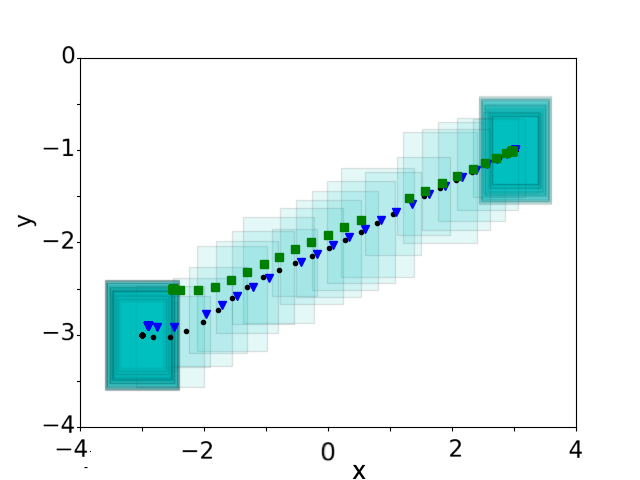
\includegraphics[width=0.4\linewidth]{figs/car_trajs.png}
    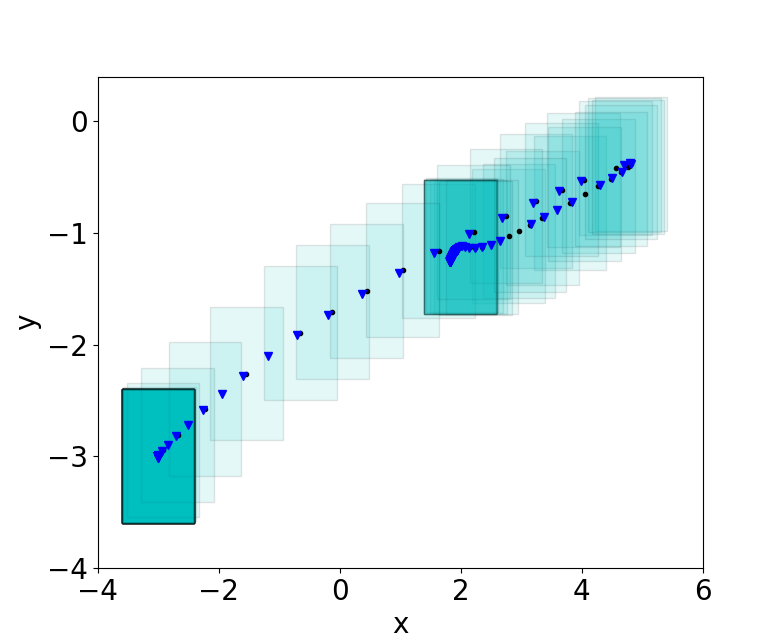
\includegraphics[width=0.4\linewidth]{figs/drone_trajs.png}
    \caption{\emph{Left}: Reachsets  for car. \emph{Right}: Reachtube for drone}
    \label{fig:dryVR}
\end{figure}